\index{Hybrid}

%\newcommand{\elist}{\epsilon}
\newcommand{\hybrid}{Hybrid}
\newcommand{\llFun}[2]{\mathsf{fun}\,#1.\,#2}
\newcommand{\llRec}[2]{\mathsf{fix}\,#1.\,#2}
\newcommand{\llrec}[1]{\ikw{fix} \  x\, .\, #1}
\newcommand{\ikw}[1]{\ensuremath{\mathsf{#1}}}
\newcommand{\hastype}{\mathrel{:}}
\newcommand{\slvdn}[3]{{#1}\rhd_{{#2}} {#3}}

\begin{figure}    \setlength{\unitlength}{4144sp}  \begingroup\makeatletter\ifx\SetFigFont\undefined
    \def\x#1#2#3#4#5#6#7\relax{\def\x{#1#2#3#4#5#6}}  \expandafter\x\fmtname xxxxxx\relax \def\y{splain}  \ifx\x\y   \gdef\SetFigFont#1#2#3{    \ifnum #1<17\tiny\else \ifnum #1<20\small\else \ifnum
    #1<24\normalsize\else \ifnum #1<29\large\else \ifnum
    #1<34\Large\else \ifnum #1<41\LARGE\else \huge\fi\fi\fi\fi\fi\fi
    \csname #3\endcsname}  \else \gdef\SetFigFont#1#2#3{\begingroup \count@#1\relax \ifnum
    25<\count@\count@25\fi
    \def\x{\endgroup\@setsize\SetFigFont{#2pt}}    \expandafter\x \csname \romannumeral\the\count@
    pt\expandafter\endcsname \csname @\romannumeral\the\count@
    pt\endcsname \csname #3\endcsname}  \fi \fi\endgroup
  %\begin{picture}(4692,2010)(34,-1198) \thinlines
  \begin{picture}(0,2010)(34,-1198) \thinlines
    {\color[rgb]{0,0,0}\put(1456,269){\oval(210,210)[bl]}
      \put(1456,509){\oval(210,210)[tl]}
      \put(2821,269){\oval(210,210)[br]}
      \put(2821,509){\oval(210,210)[tr]} \put(1456,164){\line( 1,
        0){1365}} \put(1456,614){\line( 1, 0){1365}}
      \put(1351,269){\line( 0, 1){240}} \put(2926,269){\line( 0,
        1){240}} }    {\color[rgb]{0,0,0}\put(1006,-181){\oval(210,210)[bl]} \put(1006,
      59){\oval(210,210)[tl]} \put(3271,-181){\oval(210,210)[br]}
      \put(3271, 59){\oval(210,210)[tr]} \put(1006,-286){\line( 1,
        0){2265}} \put(1006,164){\line( 1, 0){2265}}
      \put(901,-181){\line( 0, 1){240}} \put(3376,-181){\line( 0,
        1){240}} }    {\color[rgb]{0,0,0}\put(556,-631){\oval(210,210)[bl]}
      \put(556,-391){\oval(210,210)[tl]}
      \put(3721,-631){\oval(210,210)[br]}
      \put(3721,-391){\oval(210,210)[tr]} \put(556,-736){\line( 1,
        0){3165}} \put(556,-286){\line( 1, 0){3165}}
      \put(451,-631){\line( 0, 1){240}} \put(3826,-631){\line( 0,
        1){240}} }    {\color[rgb]{0,0,0}\put(151,-1081){\oval(210,210)[bl]}
      \put(151,-841){\oval(210,210)[tl]}
      \put(4216,-1081){\oval(210,210)[br]}
      \put(4216,-841){\oval(210,210)[tr]} \put(151,-1186){\line( 1,
        0){4065}} \put(151,-736){\line( 1, 0){4065}} \put(
      46,-1081){\line( 0, 1){240}} \put(4321,-1081){\line( 0, 1){240}}
    %}    \put(1936,-556){\makebox(0,0)[lb]{\smash{\SetFigFont{10}{12.0}{rm}{\color[rgb]{0,0,0}\hybrid}        }}}
    }    \put(1736,-556){\makebox(0,0)[lb]{\smash{\SetFigFont{10}{12.0}{rm}{\color[rgb]{0,0,0}\hybrid}        }}}
    \put(1851,-1006){\makebox(0,0)[lb]{\smash{\SetFigFont{10}{12.0}{rm}{\color[rgb]{0,0,0}Coq}        }}}
    %\put(3376,504){\makebox(0,0)[lb]{\smash{\SetFigFont{10}{12.0}{rm}{\color[rgb]{0,0,0}Syntax:
    %        $\llFun{x}{E\ x}, \llrec{E\ x}\dots$ }        }}}
    %\put(3376,279){\makebox(0,0)[lb]{\smash{\SetFigFont{10}{12.0}{rm}{\color[rgb]{0,0,0}Semantics:
    %        typing $E\hastype t$,\dots}        }}}

    \put(3601,299){\makebox(0,0)[lb]{\smash{\SetFigFont{10}{12.0}{rm}{\color[rgb]{0,0,0}          } }}} 

    %\put(3626,10){\makebox(0,0)[lb]{\smash{\SetFigFont{10}{12.0}{rm}{\color[rgb]{0,0,0}Sequent
    %        calculus: $\slvdn{\Gamma}{n}{G}$}        }}}
    \put(4051,-151){\makebox(0,0)[lb]{\smash{\SetFigFont{10}{12.0}{rm}{\color[rgb]{0,0,0}}        }}}
    %\put(4000,-421){\makebox(0,0)[lb]{\smash{\SetFigFont{10}{12.0}{rm}{\color[rgb]{0,0,0}Meta-language:
    %        quasi}        }}}
    %\put(4000,-601){\makebox(0,0)[lb]{\smash{\SetFigFont{10}{12.0}{rm}{\color[rgb]{0,0,0}
    %        datatype for
    %        a $\lambda$-calculus}        }}}
    %\put(4500,-871){\makebox(0,0)[lb]{\smash{\SetFigFont{10}{12.0}{rm}{\color[rgb]{0,0,0}Ambient
    %        logic:}        }}}
    %\put(4500,-1071){\makebox(0,0)[lb]{\smash{\SetFigFont{10}{12.0}{rm}{\color[rgb]{0,0,0}
    %        tactics/simplifier}        }}}
    %\put(4500,-1271){\makebox(0,0)[lb]{\smash{\SetFigFont{10}{12.0}{rm}{\color[rgb]{0,0,0}
    %        (co)induction}        }}}
    %\put(1800,344){\makebox(0,0)[lb]{\smash{\SetFigFont{10}{12.0}{rm}{\color[rgb]{0,0,0}Object
    \put(1500,344){\makebox(0,0)[lb]{\smash{\SetFigFont{10}{12.0}{rm}{\color[rgb]{0,0,0}Object
            logic}        }}}
    \put(1400,-106){\makebox(0,0)[lb]{\smash{\SetFigFont{10}{12.0}{rm}{\color[rgb]{0,0,0}Specification
            logic}        }}}
  \end{picture}
  \caption{Architecture of the Hybrid system}
  \label{fig:arch}
\end{figure}


\begin{figure}
\begin{center}
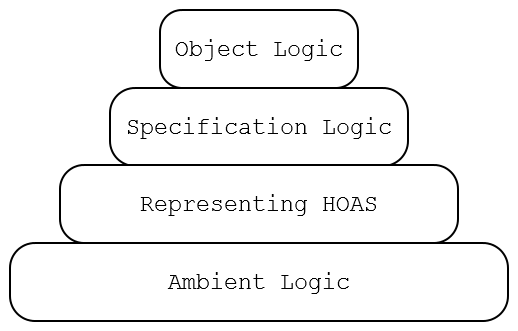
\includegraphics[height=5cm]{HybridFig.png}
\caption{High-Level Hybrid Structure \label{fig:hybrid}}
\end{center}
\end{figure}

%Recall from Chapter~\ref{ch:intro}, Hybrid is a two-level logical framework implementing operators that allow higher-order abstract syntax (HOAS) encodings of object logics (OLs) to be expressed.
%A logic that we wish to study using these systems is called an object logic (OL).
%Hybrid is implemented as a library in the interactive theorem proving language Coq, thus making it relatively easy to modify and extend the reasoning power by the addition of new intermediate logics called specification logics. One can choose the simplest specification logic necessary for the present task, or possibly a combination of more than one depending on the OL to be encoded. 
In this chapter each layer of Hybrid will be explored to provide more intuition on how it is constructed and used. This explanation will be driven by an analogy, for use as an aid to both memory and understanding of the system.

The orientation of the layers is as in Figure~\ref{fig:hybrid}. We will first consider the top layer, the object logic, in Section~\ref{sec:hybridol} with an example to motivate what we are trying to accomplish. Next we will consider each layer bottom-up, beginning with the ambient logic in Section~\ref{sec:hybridcoq}, then the higher-order abstract syntax layer in Section~\ref{sec:hybridhoas}. Continuing up the stack we next come to the specification logic. Since much of the work presented later is on the implementation and metatheory of the specification logic required for our motivating example of Section~\ref{sec:hybridol}, we will not see details of the specification logic here. Rather, Section~\ref{sec:hybridsl} will illustrate the benefit a specification logic adds to Hybrid and reinforce its necessity. This will be followed by another look at the object logic in Section~\ref{sec:hybrid_ol_imp}, but this time we will be focusing on implementation details with the rest of the system in place. To conclude this chapter, Section~\ref{sec:hybridcompare} will compare Hybrid with alternative architectures for systems intended to reason about object logics using HOAS.

\section{Object Logics}
\label{sec:hybridol}
\index{object logic}

\begin{sidestory}
Suppose we wish to study flowers and create things with them. Then we need to be able to grow flowers.
\end{sidestory}

Suppose we wish to prove something about a programming language or logic, the OL. This language will have rules expressing syntax and semantics that we need to encode in some proof assistant so that we can reason about it. It is also necessary to define the judgments of this language so that we can make claims about the OL.

%\subsection{Example OL}
\begin{expl}[Object Logic: Equivalence of Named and Nameless \lambda-terms]

We consider one of the examples presented in~\cite{WCGN:PPDP13}. Following the presentation there, we can define a syntax and rules expressing direct and de Bruijn representations of untyped $\lambda$-terms. By direct we mean the standard notation for $\lambda$-terms where abstractions reference a named variable that may be used in the body of the abstraction. De Bruijn indices~\cite{debruijn}\index{de Bruijn indices} are a nameless representation of \lambda-terms where rather than using variable names, a natural number is used for occurrences of a variable.

Let $n$ represent a natural number, $x$ a variable, and $e$ and $d$ represent direct and de Bruijn representations, respectively. Then the following are grammars for these $\lambda$-terms:
\begin{align*}
e &::= x \;\; | \;\; \lambda x . e \;\; | \;\; e \; e \\
d &::= n \;\; | \;\; \lambda d \;\; | \;\; d \; d
\end{align*}
A natural number $n$ in the grammar for de Bruijn terms $d$ serves as a pointer to the abstraction bounding that variable. This representation of \lambda-terms is more efficient for computation as we can avoid issues surrounding bound variable names. The $\lambda$-term $\lambda x . \lambda y . x \; y$ can be written using de Bruijn indices as $\lambda \; (\lambda \; (2 \; 1))$. The number $2$ refers to the outer binder (it is contained in two abstractions) and $1$ refers to the inner binder.

An example property we might want to prove is that these two representations are equivalent (or seen another way, to construct equivalent $\lambda$-terms in these different forms). This logic has a judgment to say that \lambda-term $e$ is equivalent to de Bruijn term $d$ at depth $n$, written $e \equiv_n d$. There are three inference rules expressing equivalence of these two kinds of terms, one for each of application, abstraction, and variables, seen below.
$$
\inferH[\rl{hodb\_app}]{\dyncon{} \vdash e_1 \; e_2 \equiv_n d_1 \; d_2}{\dyncon{} \vdash e_1 \equiv_n d_1 & \dyncon{} \vdash e_2 \equiv_n d_2}
$$

$$
\inferH[\rl{hodb\_abs}]{\dyncon{} \vdash \lambda x . e \equiv_n \lambda d}{\dyncon{} , x \equiv_{n+k} k \vdash e \equiv_{n+1} d}
$$

$$
\inferH[\rl{hodb\_var}]{\dyncon{} \vdash x \equiv_{n+k} k}{x \equiv_{n+k} k \in \dyncon{}}
$$

Applications in the two notations are considered equivalent under $n$ abstractions if their corresponding components are. The rule \rl{hodb\_abs} is more complicated to understand due to an additional assumption in the context of the premise of the rule. Informally, this rule says if whenever assuming variable $x$ is equivalent to index $k$ at depth $n + k$ it can be shown that the bodies of the \lambda-terms $e$ and $d$ are equivalent at depth $n + 1$, then we can conclude that the abstractions $\lambda x . e$ and $\lambda d$ are equivalent at depth $n$. As an illustration of how to use this system, we will see how to prove $\vdash \lambda x . \lambda y . x \; y \equiv_0 \lambda \; (\lambda \; (2 \; 1))$ (i.e. these two \lambda-terms are equivalent under zero additional abstractions).

\paragraph{Claim:} $\vdash \lambda x . \lambda y . x \; y \equiv_0 \lambda \; (\lambda \; (2 \; 1))$

\begin{proof}

Observe that by the \rl{hodb\_var} rule, both sequents below are provable.
\begin{align}
x \equiv_{2} 2 , y \equiv_{2} 1 \vdash x \equiv_{2} 2 \label{eqn:olex1} \\
x \equiv_{2} 2 , y \equiv_{2} 1 \vdash y \equiv_{2} 1 \label{eqn:olex2}
\end{align}
This requires $n=0$ and $k=2$ in~\eqref{eqn:olex1} and $n = k = 1$ in~\eqref{eqn:olex2}. Using the rule \rl{hodb\_app} with~\eqref{eqn:olex1} and~\eqref{eqn:olex2} we derive the sequent
\begin{align}
x \equiv_{2} 2 , y \equiv_{2} 1 \vdash x \; y \equiv_{2} 2 \; 1 \label{eqn:olex3}
\end{align}
Reviewing our claim, we are proving an equivalence of abstractions. The \rl{hodb\_abs} rule is used on~\eqref{eqn:olex3} with $k = 1$.
\begin{align}
x \equiv_{2} 2 \vdash \lambda y . x \; y \equiv_{1} \lambda \; (2 \; 1)
\end{align}
We apply \rl{hodb\_abs} again, this time with $k = 2$.
\begin{align}
\vdash \lambda x . \lambda y . x \; y \equiv_0 \lambda \; (\lambda \; (2 \; 1))
\end{align}
We have derived the sequent claimed provable, so this proof is complete.

\end{proof}

Notice that the $\lambda$ on the left of the equivalence in the conclusion of the rule $\rl{hodb\_abs}$ is a binding operator. This observation will be important when we see how to represent untyped $\lambda$-terms using HOAS in Hybrid in Section~\ref{sec:hybridhoas} and then implement this OL in Section~\ref{sec:hybrid_ol_imp}.

\end{expl}

%A few observations should be made about the rule $\equiv_{\mathit{abs}}$ before moving on. First, there is a binding operator in the conclusion of this rule. A standard abstract syntax encoding of this rule would need to reason about variable naming issues such as \alpha-conversion, \beta-reduction and managing the names of free and bound variables. Second, this rule has a premise with a variable $k$ that is only used in the context of assumptions. In the encoding this will be a parametric judgment and we will have some local quantification in the context of assumptions of this sequent (*TODO: okay? trying to motivate this example). The first observation is justification for encoding in a system using HOAS and the second necessitates the specification logic presented later.

%We have presented a logic but have so far ignored the issue of where and how we will encode it to reason about it formally.

\section{Ambient Logic}
\label{sec:hybridcoq}
\index{ambient logic}
\index{reasoning logic}

\begin{sidestory}
We can plant seeds in the ground and use the natural resources around us to reach our goal. The sun will provide energy and rain will give water.
\end{sidestory}

The ambient logic (also known as the reasoning logic or the meta-meta-logic) is the layer of the system that everything else is defined in. It is an implementation of a logic and so has its own reasoning rules and allows us to define other reasoning systems within it. In our case, this is \cic{} and its implementation in Coq. This is the lowest reasoning level we consider carefully as part of our system; we will not be concerned with lower-level details of the implementation of \cic{} or its compilation. Chapter~\ref{ch:coq} covered all aspects of Coq, the ambient logic of Hybrid, that are necessary for understanding the contributions later in this thesis.

Existing theorem proving systems are an ideal tool to allow a language and its judgments to be encoded without building extra infrastructure. Hybrid is a Coq library (a collection of Coq files), so it is relatively easy to make modular updates to the system and to add new intermediate reasoning layers called specification logics, as will be explained in Section~\ref{sec:hybridsl}.
%Further benefits to using Coq include
Hybrid can also make use of the inductive and interactive reasoning tools of Coq as well as existing Coq libraries.

\section{Representing Higher-Order Abstract Syntax in Hybrid}
\label{sec:hybridhoas}
\index{higher-order abstract syntax}

\begin{sidestory}
As our aspirations continue to grow, we find it difficult to scale up our flower production. When the rain doesn't fall as we require, we manually make up for the shortfall. The task of watering every plant every day is tedious. A dedicated plot of land with an organized arrangement and an irrigation system is a solution to this problem.
\end{sidestory}

Many tedious computations are necessary for each encoding of an OL with binding structures. Examples include fresh name generation and capture-avoiding substitution. Since Hybrid is implemented in an ambient logic that is a typed \lambda-calculus, the technique of \emph{higher-order abstract syntax} (HOAS) can be used for representing OL expressions. The idea is to use the binder of \lambda-calculus, function abstraction, to represent all OL binding operators. Using HOAS one can avoid implementing logic to reason about variable naming concepts, thus inheriting the meta-level solutions to these challenges. In addition, OL renaming and substitution are handled as meta-level \alpha-conversion and \beta-reduction, respectively.

At this level we have a type \hybridtm{expr} (see Figure~\ref{fig:expr}) encoding a de Bruijn index version of the \lambda-calculus designed to be used to represent OL syntax. A parameter \hybridtm{con} is a placeholder for OL constants, to be defined for each OL. We define \hybridtm{var} and \hybridtm{bnd} to be the natural numbers. Hybrid expressions $(\hybridtm{VAR} \; i)$ and $(\hybridtm{BND} \; j)$ represent object-level free and bound variables, respectively. The constructor \hybridtm{APP} is used to build applications and \hybridtm{ABS} to build abstractions in de Bruijn notation.

\begin{figure}
\begin{lstlisting}
Inductive expr : Set :=
| CON : con -> expr
| VAR : var -> expr
| BND : bnd -> expr
| APP : expr -> expr -> expr
| ABS : expr -> expr.
\end{lstlisting}
\caption{Terms in Hybrid \label{fig:expr}}
\end{figure}

Note that \hybridtm{con} is an implicit parameter in the environment it is defined in; uses outside of this environment must explicitly state this parameter (e.g. \sltm{expr con} instead of \sltm{expr}). A type to be given to this placeholder is defined for each OL. For example, the OL in Section~\ref{sec:hybridol} will have constants for application and abstraction for each kind of \lambda-term and a constant for variables in de Bruijn terms. These will be defined as an inductive type that is then used to instantiate the type \hybridtm{expr} for this particular OL. This example is implemented in Section~\ref{sec:hybrid_ol_imp}.

Object-level binding operators are encoded in HOAS using the Hybrid operator $\hybridtm{lambda} : (\hybridtm{expr con} \rightarrow \hybridtm{expr con}) \rightarrow \hybridtm{expr con}$ which is the meta-level binder defined in the Hybrid library. When using it to encode HOAS, the expanded definition is the underlying de Bruijn notation using only the constructors of \hybridtm{expr}. Although a Hybrid user never sees the expanded form and only works at the HOAS level. As an example, consider the untyped \lambda-term $(\lambda x . \lambda y . x \; y)$. We can represent this in Hybrid as $(\hybridtm{lambda} \; (\lambda x . (\hybridtm{lambda} \; (\lambda y . x \; y))))$ which expands to $\hybridtm{ABS} \; (\hybridtm{ABS} \; (\hybridtm{APP} \; (\hybridtm{BND} \; 1) \; (\hybridtm{BND} \; 0)))$. The \hybridtm{lambda} operator and the constructors of \hybridtm{expr} are used to encode OL syntax.

%Our example of Section~\ref{sec:hybridol} is continued in Section~\ref{sec:hybrid_ol_imp} where we can see how \hybridtm{lambda} is used in defining the OL constants and syntax in Figure \ref{fig:hoasdb_con}.


\section{Specification Logic}
\label{sec:hybridsl}
\index{specification logic}

\begin{sidestory}
Not all flowers will grow in the same conditions. Given any plot of land, there are many plants that will not grow there because they need specific nutrients in their soil. We can create different soil mixes depending on the needs of different classes of flowers.
\end{sidestory}

There are OL judgments that we cannot encode as an inductive type in Coq. One example is a HOAS encoding of inference rules assigning simple types to \lambda-expressions.
%The HOAS  rule for typing abstractions contains negative occurrences of this judgment, which is not allowed by the Coq type system. This can be seen in the HOAS encoding of the rule for typing abstractions.
The standard rule for typing abstractions can be seen in Figure~\ref{fig:stlctp}. Building on the example of Section~\ref{sec:introhoas}, let \coqtm{typ} be the type of OL types in the encoding in Coq. Let \coqtm{arr} be a constant of type $\coqtm{typ} \rightarrow \coqtm{typ} \rightarrow \coqtm{typ}$ representing arrow types. Recall \coqtm{tm} is the type of OL terms.
%Suppose that we have constants expressing the higher-order syntax of terms, including \coqtm{lambda} of type $(\underline{\coqtm{tm}} \rightarrow \coqtm{tm}) \rightarrow \coqtm{tm}$.
We want to define a typing predicate $\coqtm{tp} : \coqtm{tm} \rightarrow \coqtm{typ} \rightarrow \coqtm{Prop}$. Then the HOAS encoding of the rule for typing abstractions would be expressed as
\begin{align*}
\forall (T \; T' : \coqtm{typ}) \; & (E : \coqtm{tm} \rightarrow \coqtm{tm}), \\
& (\forall (x : \coqtm{typ}), \underline{\coqtm{tp} \; x \; T} \rightarrow \coqtm{tp} \; (E \; x) \; T') \rightarrow \coqtm{tp} \; (\coqtm{lambda} \; E) \; (\coqtm{arr} \; T \; T').
\end{align*}
Note that the \coqtm{tp} predicate cannot be expressed inductively because of the (underlined) \emph{negative occurrence} of the \coqtm{tp} predicate in the above formula for the typing abstraction rule. Inductive types with negative recursive occurrences is not allowed by the Coq type system.

As a solution to the problem of needing to reason about judgments that violate this strict positivity requirement, Hybrid is a two-level system. By two-level we mean an intermediate specification level is introduced between the OL encoding and the meta-levels. The specification logic is less expressive than the ambient logic, the calculus of constructions, but it allows us to encode judgments with negative occurrences.

\begin{figure}
$$
%\inferH[tp\_abs]{(\lambda x \, . \, E \; x) : (T \rightarrow T')}{\forall x , \underline{x : T} \rightarrow (E \; x) : T'}
\inferH[tp\_abs]{\dyncon{} \vdash \lambda x \, . \, E : T \rightarrow T'}{\dyncon{} , x : T \vdash E : T'}
%\inferH[tp\_abs]{\dyncon{} \vdash \mathit{tp} \; (\lambda x \, . \, E) \; (T \rightarrow T')}{\dyncon{} , \underline{\mathit{tp} \; x \; T} \vdash \mathit{tp} \; E \; T'}
$$
\centering{\caption{Typing of \lambda-calculus Abstractions \label{fig:stlctp}}}
\end{figure}

Hybrid is a Coq library and as mentioned earlier, this architectural decision makes quick prototyping of SLs possible. Another important benefit is that one can choose the simplest specification logic necessary for the present task, or possibly a combination of more than one depending on the OL to be encoded. Judgments that can be defined inductively do not need to be defined in a SL. This may simplify proofs of OL properties as the user can avoid using a more complicated logic than necessary.

The two levels of the OL and SL interact through a parameter of the SL,
$$
\sltm{prog} : \sltm{atm} \rightarrow \sltm{oo} \rightarrow \coqtm{Prop},
$$
which is used to encode inference rules for OL judgments (and thus define provability at the OL level). There are two arguments to \sltm{prog}; the first is the (atomic) inference rule conclusion of type \sltm{atm} and the second a formula of type \sltm{oo} representing the premise(s) of the rule.

We use $a$ for atoms with type \coqtm{atm} and $o$ for formulas of type \coqtm{oo}, possibly with subscripts.

In this implementation, the type \sltm{atm} is a parameter of the SL and is instantiated with an inductive type whose constructors predicates expressing the judgments of a particular OL. For instance, the definition of \coqtm{atm} for our above example might include a predicate $\oltm{hodb} : (\mltm{expr}~ \mltm{con}) \rightarrow \coqtm{nat} \rightarrow (\mltm{expr}~ \mltm{con}) \rightarrow \coqtm{atm}$ relating the higher-order and de Bruijn encodings at a given depth.

The type \sltm{oo} is the type of goals and clauses in the SL. The definition of \sltm{oo} for the SL defined later is in Figure~\ref{fig:oofig}.
\begin{figure}
\begin{lstlisting}
Inductive oo : Type :=
| atom : atm -> oo
| T : oo
| Conj : oo -> oo -> oo
| Imp : oo -> oo -> oo
| All : (expr con -> oo) -> oo
| Allx : (X -> oo) -> oo
| Some : (expr con -> oo) -> oo.
\end{lstlisting}
\centering{\caption{Type of SL Formulas \label{fig:oofig}}}
\end{figure}
The constant \sltm{atom} coerces an atom (a predicate applied to its arguments) to an SL formula. For any $\alpha$ of type \sltm{atm}, we may refer to ($\sltm{atom} \; \alpha$) as an atomic formula. The constructor \sltm{Conj} represents conjunction and \sltm{Imp} is used to build implications. Also note that in this implementation, we restrict the type of universal quantification to two types, (\mltm{expr}~ \mltm{con}) and \mltm{X}, where \mltm{X} is a parameter that can be instantiated with any primitive type; in our running example, \mltm{X} would become \coqtm{nat} for the depth of binding in a de Bruijn term. We leave out disjunction. It is not difficult to extend our implementation to include disjunction and quantification (universal or existential) over other primitive types, but these have not been needed in reasoning about OLs.

We write \atom{a}, ($o_1$ \& $o_2$), and ($o_1 \longrightarrow o_2$) as notation for (\sltm{atom} $a$), (\sltm{Conj} $o_1$ $o_2$), and (\sltm{Imp} $o_1$ $o_2$), respectively. Formulas quantified by \sltm{All} are written $(\sltm{All}~ o)$ or $(\sltm{All}~ \lambda (x:\mltm{expr}~ \mltm{con}) \; . \; o \; x)$, where $o$ has type $\coqtm{expr con} \rightarrow \coqtm{oo}$. The latter is the $\eta$-long form with types included explicitly. The other quantifiers are treated similarly.

The type \sltm{oo} is an inductive type, so Coq will automatically generate the induction principle shown in Figure~\ref{fig:ooip} as discussed in Section~\ref{sec:coqinduction}. We can use this induction principle to prove a statement of the form $\forall (o : \sltm{oo}), P \; o$ for some $P : \sltm{oo} \rightarrow \coqtm{Prop}$. This proof will have one subcase for each constructor of \sltm{oo}.

\begin{figure}
\begin{align*}
\sltm{oo\_ind} &: \forall (P : \sltm{oo} \rightarrow \coqtm{Prop}), \\
(*\sltm{atom}*) & \qquad (\forall (a : \sltm{atm}), P (\atom{a})) \rightarrow \\
(*\sltm{T}*) & \qquad (P \; \sltm{T}) \rightarrow \\
(*\sltm{Conj}*) & \qquad (\forall (o_1 : \sltm{oo}), P \; o_1 \rightarrow \forall (o_2 : \sltm{oo}), P \; o_2 \rightarrow P \; (o_1 \& o_2)) \rightarrow \\
(*\sltm{Imp}*) & \qquad (\forall (o_1 : \sltm{oo}), P \; o_1 \rightarrow \forall (o_2 : \sltm{oo}), P \; o_2 \rightarrow P \; (o_1 \longrightarrow o_2)) \rightarrow \\
(*\sltm{All}*) & \qquad (\forall (o : \sltm{expr con} \rightarrow \sltm{oo}), (\forall (e : \sltm{expr con}), P \; (o \; e)) \rightarrow P \; (\sltm{All} \; o)) \rightarrow \\
(*\sltm{Allx}*) & \qquad (\forall (o : \sltm{X} \rightarrow \sltm{oo}), (\forall (x : \sltm{X}), P \; (o \; x)) \rightarrow P \; (\sltm{Allx} \; o)) \rightarrow \\
(*\sltm{Some}*) & \qquad (\forall (o : \sltm{expr con} \rightarrow \sltm{oo}), (\forall (e : \sltm{expr con}), P \; (o \; e)) \rightarrow P \; (\sltm{Some} \; o)) \rightarrow \\
&\forall (o : \sltm{oo}), P \; o
\end{align*}
\centering{\caption{Induction Principle for \sltm{oo} \label{fig:ooip}}}
\end{figure}

%A Hybrid SL is defined as an inductive type in Coq where each rule is represented by a constructor of the type. The constructor name is the rule name, and the type arrow is seen as implication.

A Hybrid SL is defined as an inductive type in Coq to encode a sequent calculus. Each rule of the sequent calculus is represented by a constructor of the inductive type. The constructor name is the rule name and the type arrow is used for implication from premises to conclusion. The context of the sequent is defined to behave as a set of elements of type \sltm{oo}. We write $\dyncon{}$ or $c$ for contexts.

Since we explore the SL and proofs of its structural properties in detail later when describing the contributions of this research, we cut short the discussion here. For continuity in this chapter, some notation and the meaning of provability judgments of the SL are all we need now. We write $\seqsl{o}$ to denote an SL, where $\dyncon{}$ has type \coqtm{context} and $o$ has type \coqtm{oo}. The symbol $\rhd$ is used as the SL sequent arrow.


\section{Example OL Implementation}
\label{sec:hybrid_ol_imp}

Now we can see how to encode our example syntax and judgments in Hybrid. Let \oltm{tm} represent the type of direct \lambda-terms and \oltm{dtm} represent the type of de Bruijn terms. Since these are used to form OL expressions, \oltm{tm} and \oltm{dtm} are aliases for \sltm{expr con}. Before stating the implementation of the rules of the logic, we have to define the OL constants. For direct application and abstraction we have $\oltm{hApp} : \oltm{tm} \rightarrow \oltm{tm} \rightarrow \oltm{tm}$ and $\oltm{hAbs} : (\oltm{tm} \rightarrow \oltm{tm}) \rightarrow \oltm{tm}$, respectively. Direct variables are encoded as meta-level variables. For de Bruijn application, abstraction, and variables we have $\oltm{dApp} : \oltm{dtm} \rightarrow \oltm{dtm} \rightarrow \oltm{dtm}$, $\oltm{dAbs} : \oltm{dtm} \rightarrow \oltm{dtm}$, and $\oltm{dVar} : \coqtm{nat} \rightarrow \oltm{dtm}$, respectively.

In Figure~\ref{fig:hoasdb_con} the constants of the OL are defined in the inductive type \oltm{con}. We also have the definitions of OL applications and abstractions for the direct and de Bruijn forms of \lambda-terms in terms of the OL constants and HOAS application and \hybridtm{lambda} operator. Note that in Coq, \coqtm{fun} is notation for abstractions. When we write Coq code we use this notation but when writing pretty-printed versions of the code we will use \lambda-calculus abstraction notation. For example, we often write Coq abstractions \coqtm{fun x => f x} as $\lambda x . f \; x$ because the latter is often more readable in our discussions. In Figure~\ref{fig:hoasdb_con} we can see the use of HOAS in the definition of \oltm{hAbs} where we use the Hybrid \hybridtm{lambda} operator.

\begin{figure}
\begin{lstlisting}
Inductive con : Set := 
| hAPP : con
| hABS : con
| dAPP : con
| dABS : con
| dVAR : nat -> con.

Definition hApp : tm -> tm -> tm :=
  fun (e1 : tm) =>
    fun (e2 : tm) =>
      APP (APP (CON hAPP) e1) e2. 
Definition hAbs : (tm -> tm) -> tm :=
  fun (f : tm -> tm) => 
    APP (CON hABS) (lambda f).

Definition dApp : dtm -> dtm -> dtm :=
  fun (d1 : dtm) =>
    fun (d2 : dtm) =>
      APP (APP (CON dAPP) d1) d2. 
Definition dAbs : dtm -> dtm :=
  fun (d : dtm) =>
    APP (CON cdABS) d.
Definition dVar : nat -> dtm :=
  fun (n : nat) =>
    (CON (dVAR n)).
\end{lstlisting}
\caption{Example OL: Encoding Syntax in Hybrid \label{fig:hoasdb_con}}
\end{figure}

The atomic judgment discussed for this example (equivalence between the two representations of lambda terms) is part of the inductive type \oltm{atm} defined below.
\begin{lstlisting}
Inductive atm : Set :=
| hodb : tm -> nat -> dtm -> atm.
\end{lstlisting}
The predicate \coqtm{hodb} corresponds to the infix $\equiv_n$ relation in the rules in Section~\ref{sec:hybridol} (i.e. $\coqtm{hodb} \; e \; n \; d$ is notation for $e \equiv_n d$). In the environment where the SL is defined, there are parameters \coqtm{atm} for atomic judgments of the OL, \coqtm{con} for OL constants, and \coqtm{X} for another type we wish to universally quantify over. Now the type of SL formulas with all parameters filled in is \oltm{oo atm con X}. This is the type of SL formulas at the OL level. %We define the SL parameter $X$ used for quantification over primitive types as $\coqtm{nat}$ for this OL.

The rules shown in Section~\ref{sec:hybridol} can now be defined in Hybrid using HOAS and a SL. More specifically, we can now define the inductive type \sltm{prog} as shown in Figure~\ref{fig:hoasdb_prog}, where we see the HOAS encoding of the rules in Section~\ref{sec:hybridol}. The inductive type \coqtm{prog} has a constructor for each of the inference rules \rl{hodb\_app} and \rl{hodb\_abs}. As we will see, the \rl{hodb\_var} rule is not represented explicitly because it is taken care of at the level of the SL. The first argument to \coqtm{prog} is an atomic OL inference rule conclusion and the second argument is a formula to encode the premises of the same OL inference rule. The Coq notation for \atom{a} is \coqtm{<<a>>}.

\begin{figure}
\begin{lstlisting}
Inductive prog : atm -> oo atm (expr con) X -> Prop :=
| hobd_app : forall (e1 e2 : tm) (n : nat) (d1 d2 : dtm),
   prog (hodb (hApp e1 e2) n (dApp d1 d2))
    (<<hodb e1 n d1>> & <<hodb e2 n d2>>)
| hodb_abs : forall (f : tm -> tm) (n : nat) (d : dtm),
   abstr f ->
   prog (hodb (hAbs f) n (dAbs d))
    (All (fun (x : tm) =>
     (Allx (fun (k : X) => <<hodb x (n + k) (dVar k)>>)) --->
       <<hodb (f x) (n + 1) d>>)).
\end{lstlisting}
\caption{Example OL: Encoding OL Inference Rules \rl{hodb\_app} and \rl{hodb\_abs} in Hybrid \label{fig:hoasdb_prog}}
\end{figure}

An example theorem for this OL is to prove that the judgment $\oltm{hodb}$ is deterministic in its first and third arguments (and thus the relational definition of the rules represents a function). To do this we want to prove the two theorems below (where $=$ is equality in the ambient logic).

\begin{prop}[\oltm{hodb\_det1}]
\label{thm:hodb_det1}
\begin{align*}
& \forall (\dyncon{} : \mathtt{context}) (e : \mathtt{tm}) (d_1 \; d_2 : \mathtt{dtm}) (n : \mathtt{nat}), \\
& \qquad \seqsl{\atom{\mathtt{hodb} \; e \; n \; d_1}} \rightarrow \seqsl{\atom{\mathtt{hodb} \; e \; n \; d_2}} \rightarrow d_1 = d_2.
\end{align*}
\end{prop}

\begin{prop}[\oltm{hodb\_det3}]
\label{thm:hodb_det3}
\begin{align*}
& \forall (\dyncon{} : \mathtt{context}) (e_1 \; e_2 : \mathtt{tm}) (d : \mathtt{dtm}) (n : \mathtt{nat}), \\
& \qquad \seqsl{\atom{\mathtt{hodb} \; e_1 \; n \; d}} \rightarrow \seqsl{\atom{\mathtt{hodb} \; e_2 \; n \; d}} \rightarrow e_1 = e_2.
\end{align*}
\end{prop}

To prove these in Hybrid, we must first define a SL that is able to reason about this OL. Once we have defined the SL, using it and the encoding of the OL just described, we will be ready to prove the above propositions. As of this writing, these theorems are not proven in Hybrid.

%\begin{theorem}[\oltm{hodb\_det3}]
%\end{theorem}

\section{Comparison to Other Architectures}
\label{sec:hybridcompare}

\begin{sidestory}
Our approach to growing flowers is not the only solution. One alternative is to build a factory specializing in the production of flowers. This would give us full control over lighting, water, and soil composition; but the startup costs are high and modifications can be prohibitively expensive.
\end{sidestory}

Other systems use HOAS for encoding and reasoning about OLs with binders but different choices are made in the implementation of these systems. We will briefly look at the features of the two most closely related systems, Abella~\cite{Gacek:IJCAR08} and Beluga~\cite{Pientka:IJCAR10}, and compare these systems to Hybrid. These three systems, along with Twelf~\cite{TwelfSP}, are compared in detail using benchmark problems in~\cite{FMP:JAR15}.

One feature that sets Hybrid apart from these systems is that Hybrid is a library in an existing theorem proving system while Abella, Beluga, and Twelf are special-purpose theorem proving systems built for reasoning about OLs using HOAS. Using Coq means we can trust the proofs without having to develop extra infrastructure. These proofs can be independently checked because a proof term is a \lambda-term; a proof check is a type check in the Calculus of Constructions, a trusted and well studied theoretical foundation for our work. The trade-off is less control over the reasoning logic of Hybrid and more levels of encoding.

\paragraph{Abella}
\index{Abella}

Abella is an interactive proof environment using the special-purpose $\mathcal{G}$ logic as its reasoning logic. $\mathcal{G}$ is intuitionistic, predicative, higher-order, and has fixed-point definitions for atomic predicates. It also allows mathematical induction (over natural numbers). Infrastructure for reasoning using HOAS is built-in to this logic. Like Hybrid, it is a two-level logical framework. In contrast, since it is a special-purpose system for reasoning about OLs, only one SL is used by the system at a time; to use a different SL the system must be updated. Hybrid is a Coq library so multiple SLs can can be available for use by any OL.

Abella is a tactic-based interactive theorem prover. This is the same style used when using the interactive proof environment in Coq, but the crucial difference is that on completion of a Coq proof the system generates a proof term. This is an object that can be checked independent of the implementation of \cic{} or Coq. This means that rather than trusting the implementation of a language and the tactics, we are provided evidence on completion of the proof. Since Hybrid is implemented in Coq, we have access to proof terms once a theorem is proven. This is not the case in Abella.

An advantage to Abella is that is has the \nabla-quantifier, a new specialized quantifier providing better direct reasoning about binding in OLs. This allows Abella to prove some properties about OLs that cannot be proven in Hybrid until we implement \nabla.

\paragraph{Beluga}
\index{Beluga}

Beluga is also a logical framework for reasoning about OLs using HOAS. The reasoning logic in this system is contextual LF; it supports reasoning over contexts. It is more specialized for reasoning with HOAS than Hybrid is. It implements a type theory instead of a logic.

In Beluga, some metatheory about contexts (e.g. the structural rules of weakening, contraction, and exchange in sequent calculi) is implicit. This means that it is built-in to the implementation rather than being axioms of a logic or proven to be admissible as rules. The benefit of this choice is it is not necessary to prove theses structural rules. The argument against this is that it requires more trust from the user. It is necessary to trust the implementation of the system rather than being able to see how the rules are defined to be axiomatic or proven to be admissible.